This chapter provides discussion of load balancer suitable for container clusters.
First the author discusses problems of conventions architecture in Section~\ref{problem_k8s}.
Then the author proposes the best one in Section~\ref{proposed_arch}.
After that the author discusses inplementation of  a portable and redundant load balancer in Section~\ref{portable_lb}. 


\section{Conventional Architecture}\label{problem_k8s}

\begin{figure}
  \centering
  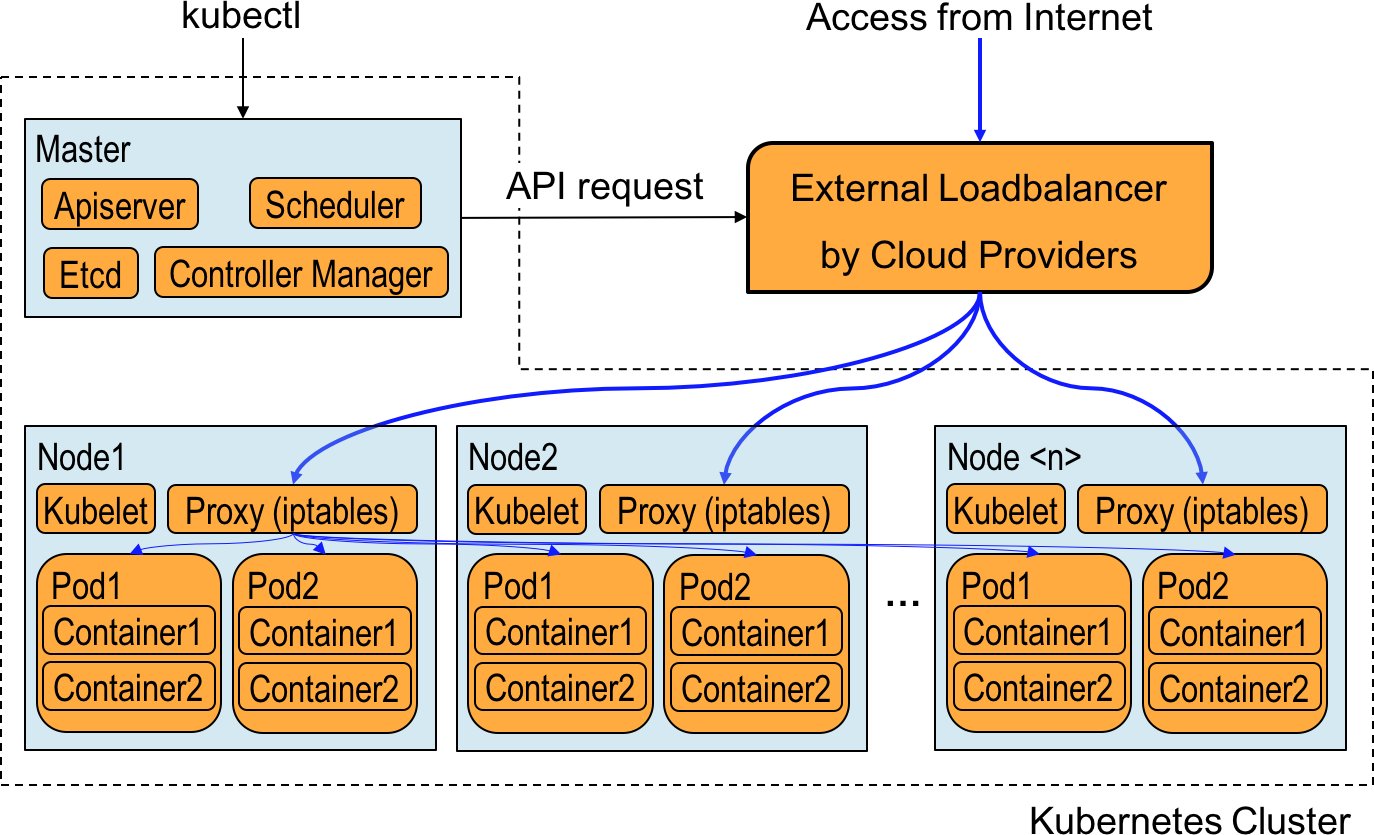
\includegraphics[width=0.8\columnwidth]{Figs/K8sConventional}
  \caption{Conventional architecture of a Kubernetes cluster.}
  \label{fig:K8sConventional}
\end{figure}

The problem of Kubernetes is its partial support for the ingress traffic routing.
Figure~\ref{fig:K8sConventional} shows an exemplified Kubernetes cluster.
A Kubernetes cluster typically consists of a master and nodes. They can be physical servers or VMs.
On the master, daemons that control the Kubernetes cluster are typically deployed. 
These daemons include, apiserver, scheduler, controller-manager and etcd. 
On the nodes, the kubelet daemon will run {\it pods}, depending the PodSpec information obtained from the apiserver on the master.
A {\em pod} is a group of containers that share the same network namespace and cgroup,
and is the basic execution unit in a Kubernetes cluster.

When a service is created, the master schedules where to run {\em pods} and kubelets on the nodes launch them accordingly.
At the same time, the master sends out requests to cloud provider's API endpoints, asking them to set up external cloud load balancers that distribute ingress traffic to every node in the Kubernetes cluster.
The proxy daemon on the nodes also setup iptables DNAT\cite{MartinA.Brown2017} rules. 
The Internet traffic will then be evenly distributed by the cloud load balancer to nodes, 
after which it will be distributed again by the DNAT rules on the nodes to the designated {\em pods}. 
The returning packets follows the exact same route as the incoming ones.

This architecture has the followings problems: 
1) There must exist cloud load balancers whose APIs are supported by the Kubernetes daemons.
There are numerous load balancers which is not supported by the Kubernetes.
These include the bare metal load balancers for on-premise data centers.
2) Distributing the traffic twice, first on the external load balancers and second on each node, complicates the administration of packet routing. 
Imagine a situation in which the DNAT table on one of the nodes malfunctions.
In such a case, only occasional timeouts would be observed, which would make it very difficult to find out which node was malfunctioning.   

Regarding the first problem, if there is no load balancer that is not supoorted by Kubernetes, users must set up the routing manually depending on the infrastructure.
The traffic would be routed to a node then distributed by the DNAT rules on the node to the designated {\em pods}.
However, this approach significantly degrades the portability of container clusters.

In short, 1) Kubernetes can be used only in limited environments where the external load balancers are supported, and 2) the routes incoming traffic follow are very complex.
In order to address these problems, the author proposes a containerized software load balancer 
that is deployable in any environment even if there are no external load balancers.

\section{Proposed Load Balancer}\label{proposed_arch}

\begin{figure}
  \centering
  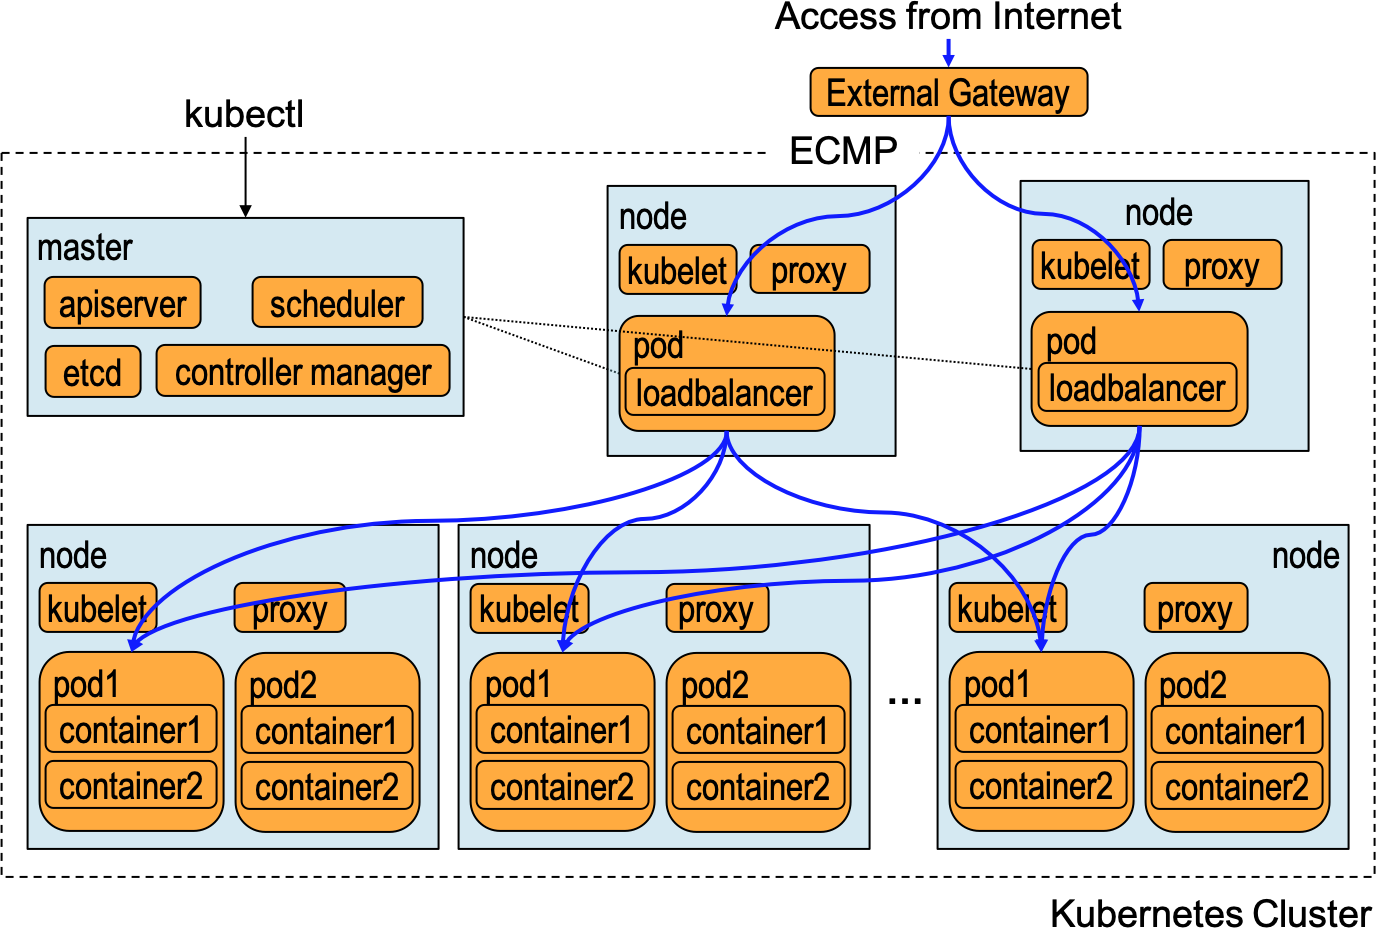
\includegraphics[width=0.8\columnwidth]{Figs/K8sProposed}
  \caption{Kubernetes cluster with proposed load balancer.}
  \label{fig:K8sProposed}
\end{figure}

The author proposes a load balancer architecture, where a cluster of load balancers are deployed as a cluster of containers.
Figure~\ref{fig:K8sProposed} shows the proposed laod balancer architecture for Kubernetes,
which has the following characteristics;
1) Each load balancer itself is run as a {\em pod} by Kubernetes. 
2) Load balancing tables are dynamically updated based on information about running {\em pods}.
3) There exist multiple load balancers for redundancy and scalability.
4) The routes to existing load balancers in the upstream router are updated dynamically using standard network protocol.

Containerized load balancer can run in any environment including on-premise data centers if only they use Linux systems.
As a result, load balancers can share the server pool with web containers.
Users can utilize existing servers rather than buying dedicated hardware.

In the case of conventional architecture, cloud load balancer distributed ingress traffic to every node and then internal load balancers based on iptables DNAT forwarded the packet again to running pods.
However, in the case of the proposed load balancers, the ingress traffic is directly routed to the running {\em pods}.
As a result, the route becomes simpler and hence finding malfunctions becomes easier than the conventional architecture.

Because a cluster of load balancer containers is controlled by a container orchestrator, it can scale the size of the cluster depending on the demand.
Furthermore, Kubernetes always tries to maintain the number of load balancer containers at the number specified by the administrator.
If a single container fails, Kubernetes schedule and launch another one on a different node, which provides the resilience to failures.

The routes to the load balancers are automatically updated through the standard protocol. 
Users do not need to manually add the route every time new load balancer container is launched, as is the case in the conventional architecture.

\FloatBarrier

\section{Implimentation}\label{sec:poc}

\subsection{General}

\begin{figure}[tb]
\begin{center}
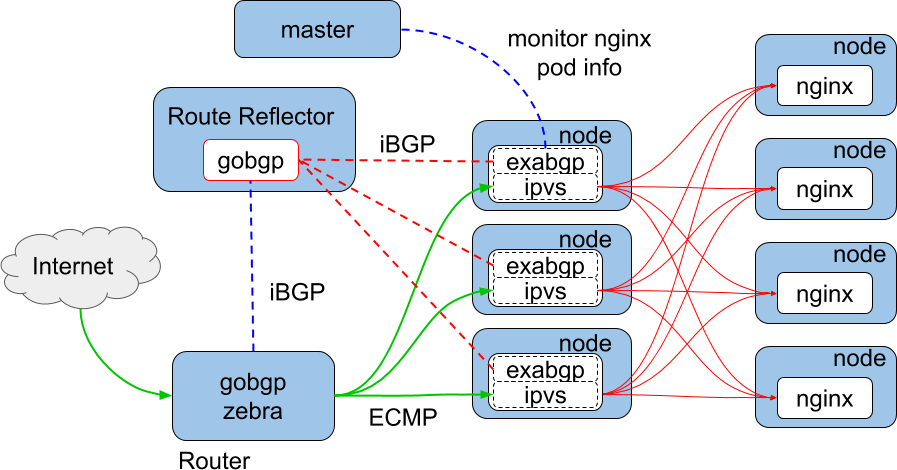
\includegraphics[width=0.8\columnwidth]{Figs/poc.png}
\end{center}
\caption{Proof of concept system}
\centering\parbox[c]{0.9\columnwidth}{
  An experimental container cluster with proposed redundant software balancers.
  The master and nodes are configured as Kubernetes's master and nodes on top of conventional Linux boxes, respectively.
  The route reflector and the upstream router are also conventional Linux boxes.
}
\label{fig:poc}
\end{figure}

Fig.~\ref{fig:poc} shows the schematic diagram of proof of concept load balancer cluster system.
%
Each load balancer pod consists of an exabgp container and an ipvs container.
The ipvs container is responsible for distributing the traffic toward the IP address that a service uses, to web server(nginx) pods.
The ipvs container monitors the availability of web server pods and manages the load balancing rule appropriately.
The exabgp container is responsible for advertising the route toward the IP address that a service uses, to the route reflector.
The route reflector aggregates the routing information advertised by load balancer pods and advertise them to the upstream router.

All the nodes and route reflector are configured using Debian 9.5 with self compiled linux-4.16.12 kernel.  
The author also used conventional Linux box as the upstream router for testing purpose, using the same OS as the nodes and route reflector.
The version of Linux kernel needed to be 4.12 or later to support hash based ECMP routing table.
The author also needed to enable kernel config option CONFIG\_IP\_ROUTE\_MULTIPATH\cite{ipsysctl} when compiling, and set the kernel parameter fib\_multipath\_hash\_policy=1 at run time.
Although in the actual production environment, proprietary hardware router with the highest throughput is usually deployed,
we could still test some of the advanced functions by using a Linux box as the router.

The exabgp is used in the load balancer pods because of the simplicity in setting as static route advertiser.
On the other hand, gobgp is used in the router and the route reflector, because exabgp did not seem to support add-path\cite{rfc7911} needed for multi-path advertisement and Forwarding Information Base(FIB) manipulation\cite{exa-networks_2018}.
The gobgp supports the add-path, and the FIB manipulation through zebra\cite{osrg_gobgp_zebra}.
The configurations for the router is summarised in \ref{appendix:router_config}.

The route reflector also uses a Linux box with gobgp and overlay network setup.
The requirements for the BGP agent on the route reflector are dynamic-neighbours and add-paths features.
The configurations for the route reflector is summarised in \ref{appendix:route_reflector_config}.

\subsection{General1}

\begin{figure}[tb]
  \centering
  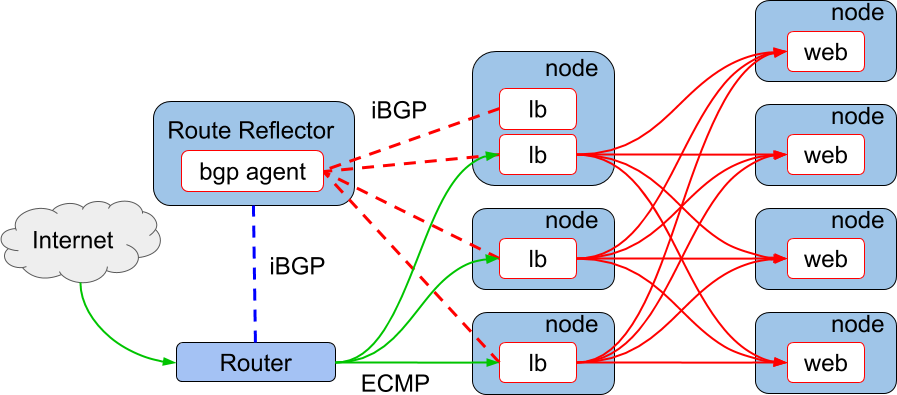
\includegraphics[width=0.8\columnwidth]{Figs/ecmp.png}
\caption{The proposed architecture of load balancer redundancy with ECMP.}

\vspace{1mm}

\begin{minipage}{0.9\columnwidth}
%\small\raggedright
  The traffic from the internet is distributed by the upstream router to multiple of lb pods using hash-based ECMP and then distributed by the lb pods to web pods using Linux kernel's ipvs.
  The ECMP routing table on the upstream router is populated using iBGP.
\end{minipage}
\label{fig:ecmp}
\end{figure}

Fig.~\ref{fig:ecmp} shows a schematic diagram to explain redundancy architecture with ECMP for the proposed load balancer.
%
The ECMP is a functionality a router often supports, where the router has multiple next hops with equal cost(priority) to a destination, and generally distribute the traffic depending on the hash of the flow five tuples(source IP, destination IP, source port, destination port, protocol).
The multiple next hops and their cost are often populated using the BGP protocol.
%
The notable benefit of the ECMP setup is the fact that it is scalable.
All the load balancers that claims as the next hop is active, i.e., all of them are utilized to increase the performance level.
Since the traffic from the internet is distributed by the upstream router, the overall throughput is determined by the router after all.
However, in practice, there are a lot of cases where this architecture is beneficial.
For example, if a software load balancer is capable of handling 1 Gbps equivalent of traffic and the upstream router is capable of handling 10 Gbps, it still is worthwhile launching 10 of the software load balancer containers to fill up maximum throughput of the upstream router.

%
We place a node with the knowledge of the overlay network as a route reflector, to deal with the complexity due to the SNAT.
The SNAT caused a problem when we tried to co-host multiple load balancer containers for different services on a single node, and let them connect the upstream router directly.
This was due to the fact that the BGP agent used in our experiment only used the source IP address of the connection to distinguish the BGP peer.
The agent behaved as though different BGP connections from different containers belonged to a single BGP session because the source IP addresses were identical due to the SNAT.

A route reflector is a network component for BGP to reduce the number of peerings by aggregating the routing information\cite{rfc4456}.
In our proposed architecture we use it as a delegater for load balancer containers towards the upstream router.

By using the route reflector, we can have the following benefits.
1) Each node can accommodate multiple load balancer containers. This was not possible when we tried to directly connect load balancers and the router through SNAT.
2) The router does not need to allow peering connections from random IP addresses that may be used by load balancer containers. Now, the router only need to have the reflector information as the BGP peer definition.

Since we use standard Linux boxes for route reflectors, we can configure them as we like;
a) We can make them belong to overlay network so that multiple BGP sessions from a single node can be established.
b) We can use a BGP agent that supports dynamic neighbor (or dynamic peer), where one only needs to define the IP range as a peer group and does away with specifying every possible IP that load balancers may use.

The upstream router does not need to accept BGP sessions from containers with random IP addresses, but only from the route reflector with well known fixed IP address. This may be preferable in terms of security especially when a different organization administers the upstream router.
Although not shown in the Fig.~\ref{fig:ecmp}, we could also place another route reflector for redundancy purpose.

%\section{Proof of concept system}\label{sec:poc}

\FloatBarrier

\subsection{BGP software container}\label{sec:bgp}

\begin{figure}[tb]

  \begin{subfigure}[t]{\columnwidth}
    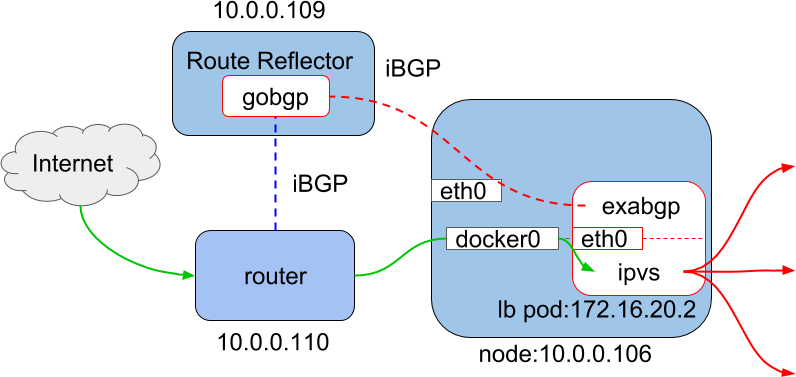
\includegraphics[width=0.9\columnwidth]{Figs/exabgp}
    \caption{}
    \label{fig:exabgp_schem}
  \end{subfigure}

  \par\bigskip

  \begin{subtable}{.9\textwidth}
    \centering
    \begin{tabular}{l}
      \hline 
      \multicolumn{1}{l}{[BGP announcement]} \\
      \hspace{15 mm} route 10.1.1.0/24 next-hop 10.0.0.106 \\
      \multicolumn{1}{l}{[Routing in node net namespace]} \\
      \hspace{15 mm} ip netns exec node ip route replace 10.1.1.0/24 dev docker0 \\
      \multicolumn{1}{l}{[Accept as local]} \\
      \hspace{15 mm} ip route add local 10.1.1.0/24 dev eth0 \\
      \hline
    \end{tabular}
    \caption{}
    \label{fig:exabgp_setting}
  \end{subtable}

  \caption{
    (a) Network path by the exabgp container. (b) Required settings in the exabgp container.
  }
  \label{fig:exabgp}
\end{figure}

In order to implement the ECMP redundancy, we also containerized exabgp using Docker.
Fig.\ref{fig:exabgp}~(\subref{fig:exabgp_schem}) shows a schematic diagram of the network path realized by the exabgp container.
We used exabgp as the BGP advertiser as mentioned earlier.
The traffic from the Internet is forwarded by ECMP routing table on the router to the node, then routed to ipvs container.

Fig.\ref{fig:exabgp}~(\subref{fig:exabgp_setting}) summarises some key settings required for the exabgp container.
In BGP announcements the node IP address, 10.0.0.106 is used as the next-hop for the IP range 10.1.1.0/24.
Then on the node, in order to route the packets toward 10.1.1.0/24 to the ipvs container, 
a routing rule to the dev docker0 is created in the node net namespace. 
A routing rule to accept the packets toward those IPs as local is also required in the container net namespace. 
A configuration of exabgp is shown in \ref{appendix:exabgp_config}.

\mytodo[inline]{Compare about OSS bgp softwares.}

\FloatBarrier

\subsection{Ipvs container}\label{sec:ipvs}

\begin{figure}
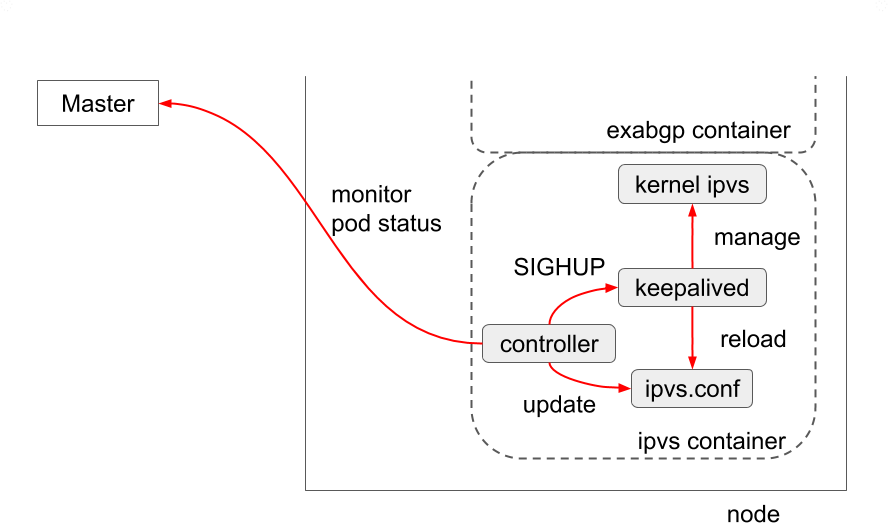
\includegraphics[width=0.8\columnwidth]{Figs/ipvs-ingress-schem}
\caption{Implementation}
\label{fig:IPVS-ingress-schem}
\end{figure}

The proposed load balancer needs to dynamically reconfigure the IPVS balancing rules whenever {\em pods} are created/deleted. 
Figure~\ref{fig:IPVS-ingress-schem} is a schematic diagram to show the dynamic reconfiguration of the IPVS rules.
Two daemon programs, controller and keepalived, run in the container inside the LB2 pod are illustrated.
The keepalived manages Linux kernel's IPVS rules depending on the ipvs.conf configuration file.
It is also capable of health-checking the life of {\em real server}, 
which is represented as a combination of the IP addresses and port numbers of the target {\em pods}. 
If the health check to a {\em real server} fails, keepalived will remove that {\em real server} from the IPVS rules.

The controller monitors information concerning the running {\em pods} of a service 
in the Kubernetes cluster by consulting the apiserver running on the master.
Whenever {\em pods} are created or deleted, the controller will automatically regenerate an appropriate ipvs.conf 
and issue SIGHUP to keepalived.
Then, keepalived will reload the ipvs.conf and modify the kernel's IPVS rules accordingly.
The actual controller\cite{ktaka_ccmp_2017_826894} is implemented using the Kubernetes ingress controller\cite{K8sIngress2017} framework. 
By importing existing Golang package, \enquote{k8s.io/ingress /core/pkg/ingress}, we could simplify the implementation, e.g. 
120 lines of code.  

Configurations for capabilities were needed in the implementation: adding the CAP\_SYS\_MODULE capability 
to the container to allow the kernel to load required kernel modules inside a container, 
and adding CAP\_NET\_ADMIN capability to the container to allow keepalived to manipulate the kernel's IPVS rules. 
For the former case, we also needed to mount the \enquote{/lib/module} of the node's file system on the container's file system.

\begin{figure}
  \centering
\begin{minipage}{0.7\columnwidth}
\begin{lstlisting}[frame=single]
  virtual_server fwmark 1 {
    delay_loop 5
    lb_algo lc
    lb_kind NAT
    protocol TCP
    real_server 172.16.21.2 80 {
      uthreshold 20000
      TCP_CHECK {
        connect_timeout 5
        connect_port 80
      }
    }
    real_server 172.16.80.2 80 {
      uthreshold 20000
      TCP_CHECK {
        connect_timeout 5
        connect_port 80
      }
    }
  }
\end{lstlisting}
\end{minipage}
\caption{An example of ipvs.conf}
\label{fig:ipvs.conf}
\end{figure}

\begin{figure}
  \centering
%\begin{minipage}{\columnwidth}
\rule{\columnwidth}{0.4pt}
\begin{verbatim}
# kubectl exec -it IPVS-controller-4117154712-kv633 -- IPVSadm -L
IP Virtual Server version 1.2.1 (size=4096)
Prot LocalAddress:Port Scheduler Flags
  -> RemoteAddress:Port Forward Weight ActiveConn InActConn
FWM  1 lc
  -> 172.16.21.2:80      Masq    1      0          0         
  -> 172.16.80.2:80      Masq    1      0          0
\end{verbatim}
\rule{\columnwidth}{0.4pt}
%\end{minipage}
\caption{Example of IPVS balancing rules}
\label{fig:IPVS rule}
\end{figure}


Figure~\ref{fig:ipvs.conf} and Figure~\ref{fig:IPVS rule} show an example of an ipvs.conf file 
generated by the controller and the corresponding IPVS load balancing rules, respectively.
Here, we can see that the packet with {\tt fwmark=1}\cite{BertHubert2002} is distributed 
to {\tt 172.16.21.2:80} and {\tt 172.16.80.2:80} 
using the masquerade mode(Masq) and 
the least connection(lc)\cite{Zhang2000} balancing algorithm.

\mytodo[inline]{Write about ingress controller implementation.}


\section{Summary}
\mytodo[inline]{Write summary for implementation.}
